%  Architecture.tex
%  Document created by seblovett on hind.ecs.soton.ac.uk
%  Date created: Thu 27 Mar 2014 10:11:44 GMT
%  <+Last Edited: Mon 28 Apr 2014 22:45:06 BST by seblovett on seblovett-Ubuntu +>
\subsection{Architecture}

Figure~\ref{fig:architecture} shows the datapath architecture of the \samurai{} processor. 
The controller has been omitted along with all control signals. 
The exception is the status register is shown for data flow as this utilises the System Bus. 
Instruction decoding is also not shown for clarity. 
All registers, buses and multiplexors are 16 bits in length unless otherwise stated. 

\begin{figure}
%%\missingfigure{Architecture diagram}
%\hspace*{-1in}
\vspace*{-1.5in}
\makebox[\linewidth]{
\centerline{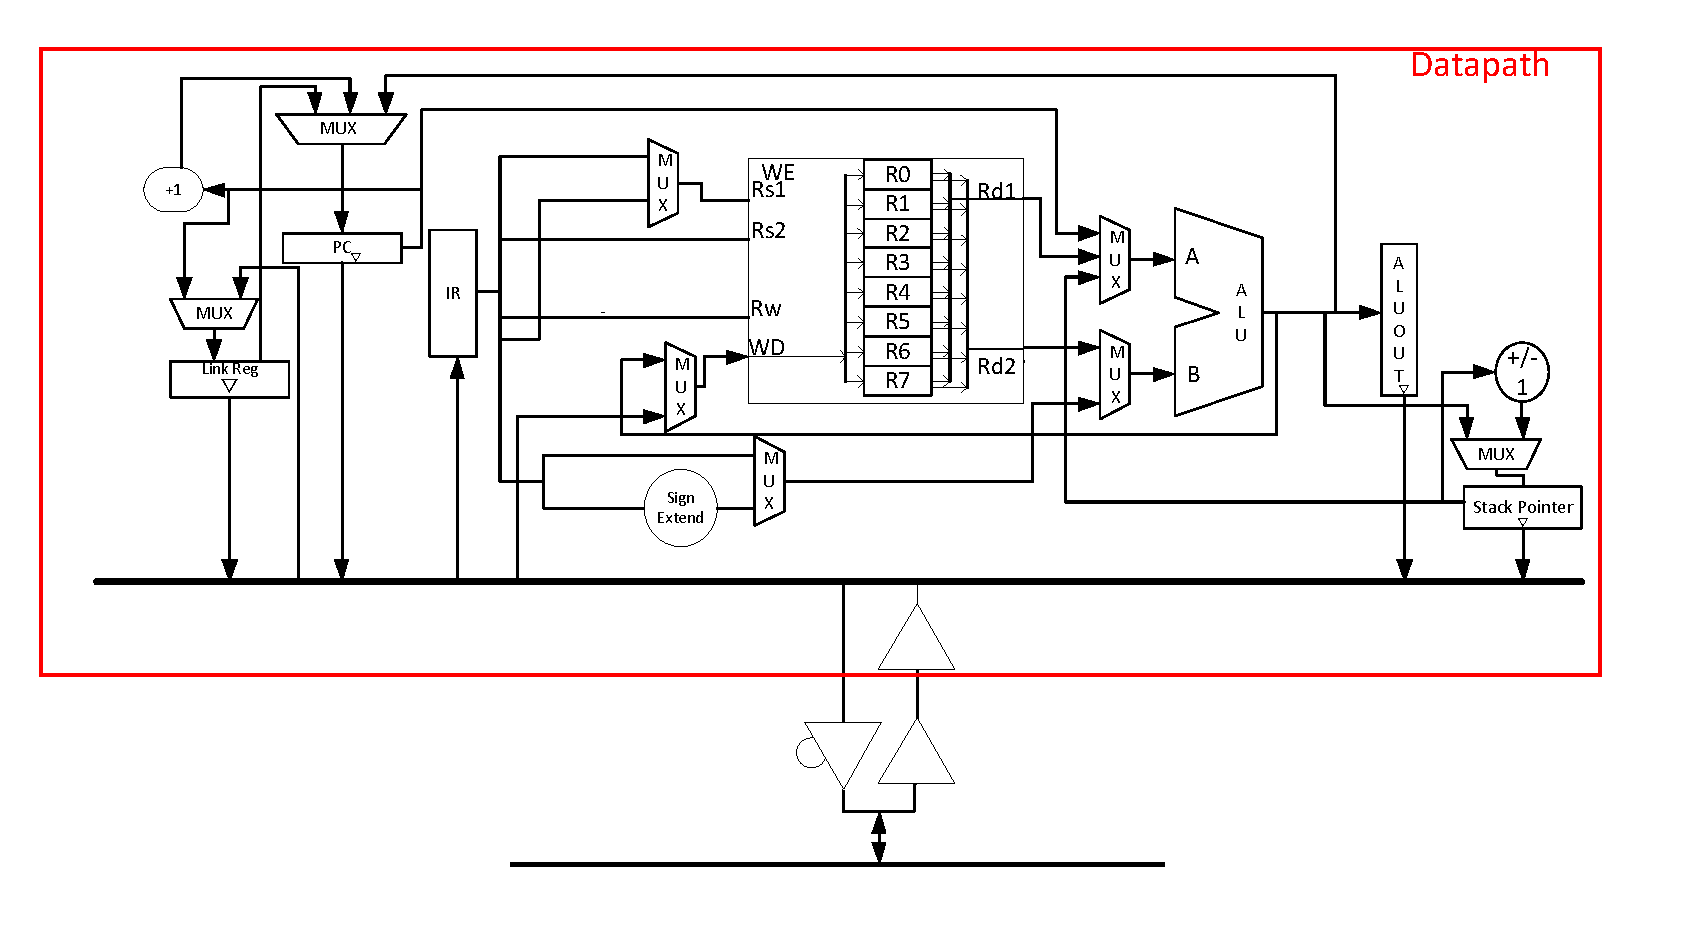
\includegraphics[angle=270,width=\textwidth-1cm]{../../Design/RandD/idea1.pdf}}
}
\caption{The Architecture diagram of the \samurai{} processor.}
\label{fig:architecture}
\end{figure}
